%%%%%%%%%%%%%%%%%%%%%%%%%%%%%%%%%%%%%%%%%%%%%%%%%%%%%%%%%%%%%%%%%%%%%%%%%%%%%%%%
%2345678901234567890123456789012345678901234567890123456789012345678901234567890
%        1         2         3         4         5         6         7         8

\documentclass[letterpaper, 10 pt, conference]{ieeeconf}  % Comment this line out if you need a4paper
\usepackage{textcomp}
\usepackage{tikz}
\usetikzlibrary{automata,positioning,arrows}

%\documentclass[a4paper, 10pt, conference]{ieeeconf}      % Use this line for a4 paper

\IEEEoverridecommandlockouts                              % This command is only needed if 
                                                          % you want to use the \thanks command

\overrideIEEEmargins                                      % Needed to meet printer requirements.

%In case you encounter the following error:
%Error 1010 The PDF file may be corrupt (unable to open PDF file) OR
%Error 1000 An error occurred while parsing a contents stream. Unable to analyze the PDF file.
%This is a known problem with pdfLaTeX conversion filter. The file cannot be opened with acrobat reader
%Please use one of the alternatives below to circumvent this error by uncommenting one or the other
%\pdfobjcompresslevel=0
%\pdfminorversion=4

% See the \addtolength command later in the file to balance the column lengths
% on the last page of the document

% The following packages can be found on http:\\www.ctan.org
\usepackage{graphics} % for pdf, bitmapped graphics files
\usepackage{epsfig} % for postscript graphics files
%\usepackage{mathptmx} % assumes new font selection scheme installed
%\usepackage{times} % assumes new font selection scheme installed
\usepackage{amsmath} % assumes amsmath package installed
%\usepackage{amssymb}  % assumes amsmath package installed
\usepackage{subcaption}
\usepackage{hyperref}

\usepackage{listings}
\usepackage{color}

% Subplotting
%\usepackage[demo]{graphicx}
%\usepackage{subfig}

\definecolor{dkgreen}{rgb}{0,0.6,0}
\definecolor{gray}{rgb}{0.5,0.5,0.5}
\definecolor{mauve}{rgb}{0.58,0,0.82}

\lstset{frame=tb,
  language=C++,
  aboveskip=3mm,
  belowskip=3mm,
  showstringspaces=false,
  columns=flexible,
  basicstyle={\small\ttfamily},
  numbers=none,
  numberstyle=\tiny\color{gray},
  keywordstyle=\color{blue},
  commentstyle=\color{dkgreen},
  stringstyle=\color{mauve},
  breaklines=true,
  breakatwhitespace=true,
  tabsize=3
}

\usepackage[T1]{fontenc}

\title{\LARGE \bf
High-Speed Autonomous Racing Engineers (H.A.R.E.) Final Report
}

\author{Mike Flanigan$^{1}$, Jack Kawell$^{2}$, Mike Ohradzansky$^{3}$, Eugene Rush$^{4}$,  and James Watson$^{5}$% <-this % stops a space
\thanks{$^{1}$ Mike Flanigan is with the Department of Computer Science, University of Colorado Boulder,
        Boulder, CO 80309, USA
        {\tt\small michael.flanigan@colorado.edu}}%
\thanks{$^{2}$Jack Kawell is with the Department of Computer Science, University of Colorado Boulder,
        Boulder, CO 80309, USA
        {\tt\small jack.kawell@colorado.edu}}%
\thanks{$^{3}$Mike Ohradzansky is with the Department of Aerospace Engineering Sciences, University of Colorado Boulder,
        Boulder, CO 80309, USA
        {\tt\small michael.ohradzansky@colorado.edu}}%
\thanks{$^{4}$Eugene Rush is with the Department of Mechanical Engineering, University of Colorado Boulder,
        Boulder, CO 80309, USA
        {\tt\small eugene.rush@colorado.edu}}%
\thanks{$^{5}$James Watson is with the Department of Computer Science, University of Colorado Boulder,
        Boulder, CO 80309, USA
        {\tt\small james.watson-2@colorado.edu}}%
}

\begin{document}

\maketitle
\thispagestyle{empty}
\pagestyle{empty}


%%%%%%%%%%%%%%%%%%%%%%%%%%%%%%%%%%%%%%%%%%%%%%%%%%%%%%%%%%%%%%%%%%%%%%%%%%%%%%%%
\begin{abstract}

This document gives an overview of the methodology implemented to accomplish the challenges presented in the Advanced Robotics course. The team was tasked with creating a $1/10^{th}$ scale autonomous car that could navigate a simple hallway course at a high speed as well as complete various other driving related challenges. This report covers our system design, which is based on a simple RC car chassis and an RGB-D camera for sensory input. The control strategy for the vehicle revolves around a Proportional-Integral-Derivative (PID) based steering control law wrapped into a Finite State Machine (FSM) architecture. Additionally, we discuss our approaches to complete each small challenge and two appendices which discuss different control methods as well as a theoretical implementation of Deep Learning (DL) for improving the vehicle's performance.

\end{abstract}


%%%%%%%%%%%%%%%%%%%%%%%%%%%%%%%%%%%%%%%%%%%%%%%%%%%%%%%%%%%%%%%%%%%%%%%%%%%%%%%%
\section{INTRODUCTION}

Cars have been around since the late 1800's, and we are beginning to enter a new era in transportation with recent developments in the self-driving car industry. Spurred by DARPA's Grand Challenge for Autonomous Vehicles in 2004, research in the field of vehicle autonomy has significantly grown with many companies, such as Tesla and Uber, trying to be the first to reach fully autonomous cars. The level of autonomy that a vehicle is able to achieve is classified into five levels. At the lower levels, some assistance may be provided to the driver of the vehicle or it may be able to take over control in certain conditions, but the driver is still required to be alert at the wheel. At the higher levels of autonomy, the vehicle should be able to navigate nearly any scenario while the driver sleeps. At level 5 autonomy, no steering wheel is needed and there are no restrictions on where and when the vehicle can drive itself. 

In the spirit of exploring the field of robotics and diving deeper into the realm of autonomous driving, a challenge has been presented to students at the University of Colorado Boulder. The challenge is to try and achieve level 2 autonomy where the vehicle is driving itself with the driver (grad students) ready to intervene in the case of an imminent crash.

\begin{figure}[h]
\begin{center}
\includegraphics[width=.48\textwidth]{Figures/group.jpg}
\caption{Group photo with final robot.}
\label{group}
\end{center}
\end{figure}

\subsection{Challenge Overview}

For CSCI-5302 Team H.A.R.E. was tasked with designing, programming, and testing an autonomous $1/10^{th}$ scale RC car. The main challenge was to autonomously navigate a specified course in the fastest time possible using only the provided sensors. In addition to the main challenge, it was required that several other smaller challenges be selected and completed. The full list of challenges team H.A.R.E chose to complete is below:

\begin{itemize}
  \item *. Complete a course lap in less than 20 seconds... and preferably faster than anyone else. 
  \item A. Detect a collision, back out, continue driving.
  \item B. Power slide around turns while racing. 
  \item B. Stop at a stop sign.
  \item C. Research and report on how deep learning could improve our car performance. 
  \item C. Implement and report on two control schemes. 
\end{itemize}

Each one of the challenges is meant to push the team and the capabilities of the autonomous car, and the team tried to select challenges that explored different branches of robotics. Being able to detect (and prevent, if possible) a collision and have the ability to recover is a useful skill for any autonomous vehicle. Power sliding requires super fine tuning of the steering controller and insight into complex vehicle dynamics. Image processing and object detection are necessary components for detecting a stop sign. Deep learning speaks for itself as a promising new field of research.

We have made the culmination of our efforts available as a public code repository. \cite{HAREproject}

\newpage
\subsection{Course Overview}

The race course for this project is a U-shaped hallway in the basement of the CU Boulder Engineering Center, specifically the Environmental Science (ECES) wing. As shown in Figure \ref{ECCR_basement_map_v2_with_photos_scale}, the course is traversed in a clockwise fashion and consists of (1) a 20 m straightaway, (2) a 90 degree right turn, (3) a 30 m straightaway section, (4) a second 90 degree right turn, and (5) and final 20 m straightaway.

\begin{figure}[h]
\begin{center}
\includegraphics[width=.48\textwidth]{Figures/ECCR_basement_map_v2_with_photos_scale.png}
\caption{Two-dimensional map of test course to scale.}
\label{ECCR_basement_map_v2_with_photos_scale}
\end{center}
\end{figure}

\section{RELATED WORK}
% MIT car stuff?
% [MIKE F IS GOING TO TAKE ON THIS SECTION]
Research on related work was done to determine what techniques and approaches could be effective for completing various challenges. Studying other projects provided a good starting direction and inspiration on various tasks. While many of the techniques went unused building an understanding of each project's domain challenges gave a nice jump start to understanding the broader scope of autonomous vehicle challenges. The below list gives an overview of the three main projects researched and some of their key aspects:
\begin{enumerate}
   \item Georgia Tech - AutoRally \cite{AutoRally}
   \begin{itemize}
        \item The AutoRally project developed perception and control algorithms for a $1/8^{th}$ scale RC car in an off-road setting.
        \item This project was of interest particularly due to its use of Model-Predictive-Control in a dynamic friction setting since drifting was a chosen challenge task. 
   \end{itemize}
   \item Berkeley Autonomous Race Car - BARC \cite{BARC}
     \begin{itemize}
        \item The BARC project is built around ROS and a $1/10^{th}$ scale rc car with a very similar sensor suite and challenge goals as the CSCI-5302 challenge.
        \item Studying the general software, control, and design architecture of this project provided a nice benchmark for similarity comparisons. 
   \end{itemize}
   \item MIT - RACECAR \cite{RACECAR}
   \begin{itemize}
        \item The MIT RACECAR project was developed first for a class and was then open sourced. It also uses ROS and a $1/10^{th}$ scale rc car. The sensor suite has the notable difference of a LIDAR however the target vehicle capabilities were similar. 
        \item The most useful takeaway from the RACECAR project was the use, understanding, and modification of the ROS simulator. This provided an invaluable testing environment for control scheme testing.  
    \end{itemize}
\end{enumerate}

Of the above projects the MIT - RACECAR project ended up lending the most valuable knowledge since it 1) provided the simulator already mentioned 2) had several similar challenge tasks that provided a good starting point for control strategies. 

\section{METHODOLOGY}
% Section for describing our approach to handling the course

\subsection{Provided Hardware}
To establish fairness in this competition, graduate student teams were all provided and limited to the hardware shown in Table \ref{table:1}. All teams received the 1/10 scale RC car with an oDroid as the compute platform and the Realsense for perception.

\begin{table}[h!]
\begin{center}
\caption{Bill of materials.}
\begin{tabular}{ p{1.2cm} p{5.0cm} p{0.4cm} }
 \hline
 Manuf      &   Part                            &   Qty \\
 \hline
 Traxxas    &   Rustler 1/10 2WD                &   1\\
 ODROID     &   XU4 with 64 GB eMMC Card        &   1\\
 Intel      &   RealSense D435                  &   1\\
 Pololu     &   18-Channel USB Servo Controller &   1\\
 Tenergy    &   2S 1800mAh NiMH Batteries       &   2\\
 Tenergy    &   2S 3000mAh NiMH Batteries       &   2\\
 \hline
\end{tabular}
\label{table:1}
\end{center}
\end{table}

\subsection{System Design}
% Brief section for describing the vehicle
% - USE THIS SECTION FOR TALKING ABOUT DESIGN PROCESS STRATEGY
% - We want a complete but succinct description of our vehicle and an accompanying image.
% - Focus on high level decisions that were made regarding sensor choices and placement. We don't need to point out every nut and bolt

The design for our vehicle is based around the Traxxas Rustler $1/10^{th}$ scale RC car chassis. A motor / ESC combo is used for spinning the rear motors of the vehicle while a single servo is used for steering the front tires. Figure \ref{iso} shows the computer aided design (CAD) model which was built by our team to the exact specifications of our parts.

\begin{figure}[h]
\begin{center}
\includegraphics[width=.48\textwidth]{Figures/ISO_view_HARE.png}
\caption{Isometric view of the vehicle done in CAD}
\label{iso}
\end{center}
\end{figure}

Our initial design strategy was to get everything mounted to the vehicle as quickly as possible so that we could begin work on getting the vehicle controlled from ROS. With this in mind, the first part which was created for the vehicle was the electronics deck seen in Figure \ref{platform}.

\begin{figure}[h]
\begin{center}
\includegraphics[width=.48\textwidth]{Figures/platform.png}
\caption{Platform deck for holding electronics.}
\label{platform}
\end{center}
\end{figure}

Quick prototyping with additive manufacturing allowed us to design, fabricate, and mount the electronics deck in a matter of days. Once we were able to mount all our electronics, such as the ODROID computer and Pololu PWM controller, we were ready to being controlling the vehicle. 

In order to facilitate quick testing of the vehicle control, a Naze32 flight control board was added to the vehicle for easy access to RC commands coming from a 2.4Ghz radio transmitter / receiver pair. The Naze32 was flashed with ROSFlight, which is an open source flight control stack for controlling multi-rotors vehicles. Being able to receive external RC commands allowed us to easily tune the steering controller so that a 0 degree commanded steering angle would drive the vehicle straight forward. We were also able to leverage switches on the transmitter to enable an e-stop for safely terminating vehicle motion and a manual control override.

To protect the steering servo during a crash, a front bumper was added to the vehicle as seen in Figure \ref{bumper}. The design of this bumper was such that it absorbed most of the impact in a head-on collision with walls and corners and would brake before any core components of the system would. This allowed us to test at high speeds without  endangering our more valuable components. Additionally, the bumper was built using 3D printing and thus could be rapidly replaced when needed.

\begin{figure}[h]
\begin{center}
\includegraphics[width=.48\textwidth]{Figures/bumper.png}
\caption{Bumper cage to absorb accidental collisions.}
\label{bumper}
\end{center}
\end{figure}

A custom camera mount was designed so that we could easily change the orientation of the RealSense camera. Our original control scheme required the camera to be mounted at a 45 degree angle relative to the front of the vehicle, while the final control scheme we went with required the camera to be pointing straight forward.

\begin{figure}[!h]
  \centering
  \begin{minipage}[b]{0.22\textwidth}
    \includegraphics[width=\textwidth]{Figures/straight-rs-mount.png}
    \caption{RealSense mount in the forward configuration.}
  \end{minipage}
  \hfill
  \begin{minipage}[b]{0.22\textwidth}
    \includegraphics[width=\textwidth]{Figures/turned-rs-mount.png}
    \caption{RealSense mount in the \textit{45\textdegree} configuration.}
  \end{minipage}
\end{figure}

\subsection{Sensors \& Data Processing} \label{lineScan}

An Intel RealSense D435i provided visual and depth data (RGB-D). The RealSense is a structured-light camera that projects two infrared patterns into the field of view of the image sensor, and calculates per-pixel depth using interferometry. Additionally, it has a full RGB camera sensor for color sensitive tasks.

Although an open-source RealSense ROS wrapper is available at \url{https://github.com/IntelRealSense/realsense-ros}, the H.A.R.E. car utilizes a lighter-weight custom ROS RealSense wrapper. This wrapper publishes a \textit{std\textunderscore{}msgs::Float32MultiArray} ROS message named \textit{/camera/depth/image\textunderscore{}rect\textunderscore{}raw} image, which is represented by the OpenCV format \textit{CV\textunderscore{}32F} and has units of meters. Input parameters include flags that control the processing and publishing of the depth image, infrared images, and RGB image.

\begin{lstlisting}
// Obtain 16-bit depth matrix
cv::Mat mat_depth_16b(Size(DEPTH_WIDTH, DEPTH_HEIGHT), CV_16U, (void*)(frame_depth.get_data()), Mat::AUTO_STEP);
// Obtain depth image (meters) for calculations
mat_depth_16b.convertTo(mat_depth_meters, CV_32F, scale);
// Copy from cv::Mat to std_msgs::Float32MultiArray
depth_msg.data.clear();
depth_msg.data.insert(depth_msg.data.end(), (float*)mat_depth_meters.datastart, (float*)mat_depth_meters.dataend);
// Publish depth image //
pub_image_depth_meters.publish(depth_msg);
\end{lstlisting}

Although such rich sensory data is useful for general navigation and perception tasks, we found it pragmatic to simplify this depth data for two reasons. The first is simply the low-powered nature of our ODROID XU-4 platform which limits single-threaded performance compared to a desktop type platform. Secondly, by subsampling from the full depth image, we are able to render a less noisy frame for our controller to act on. The main output of this custom wrapper is the depth image represented as the MultiArray mentioned above.

We reduced the depth image into binned ``line scans'' that have an output that mimics that of a Light Detection and Ranging (LIDAR) sensor.  (See Figure \ref{scanArr})  A ROS node takes as input depth images ($640 \times 360$ resolution) from the RealSense at a rate of 60 frames per second (FPS).  From this image we select 3 rows of the depth image.  These rows need not be contiguous and they are settable at run-time.  The pixels of each row are separated into $n$ bins with roughly equal pixel widths ($n=100$ for our system).  The value of each element in the line scan is the average of all the depth pixels in the bins across the 3 selected rows, yielding a 1-dimensional array of averaged depth values from left to right across the 91\textdegree \ horizontal field of view (FOV). This scheme has several advantages.  The first is that noise is averaged out within each bin: each bin is the average of about 21 depth pixels.   Secondly, we can select rows that are vertically spaced so that features that exist at a certain level above ground, such as windows, do not present an incorrect perception of the hallway to the system.  The most important advantage of the line scan is that it represents the 2-dimensional accessible driving space in a form that is very compact but still sufficient for control at high speed.  Figure \ref{scanCart} shows that the line scan contains sufficient environmental data to accomplish the racing task.

\begin{figure}[t]
    \centering
    \includegraphics[width=\columnwidth]{Figures/scanArr.png}
    \caption{Typical line scan recorded from the robot during race task execution (distance [m] versus array index), note the entry-way feature, seen as a discontinuity in the curve}
    \label{scanArr}
\end{figure}

\begin{figure}[b]
    \centering
    \includegraphics[width=\columnwidth]{Figures/scanCart.png}
    \caption{The same scan as Figure \ref{scanArr}, with each of the scan points projected to 2D Cartesian space with the depth sensor at <0,0> and $+y$ as the forward direction.}
    \label{scanCart}
\end{figure}

Our system reduces the depth image to two such line scans: one that samples 3 widely-spaced rows above level to capture the overall shape of the hallway (for control), and one that samples 3 tightly-spaced rows below level to capture obstacles very near to the robot (for collision avoidance).

For the stop sign detection challenge we also needed to be able to read the RGB image data from the RealSense. Because of our limited single-threaded performance, we decided to implement this functionality in a separate light weight RealSense wrapper ROS node. This node was only responsible for reading in a stream of RGB images ($640 \times 360$ resolution) at a rate of 30FPS. Though a higher framerate would theoretically increase the accuracy of stop sign detection, our compute resources limited us to only 30FPS for RGB images instead of the 60FPS for depth. This however did not negatively affect the results of our stop sign detection. Similarly to the depth RealSense wrapper, this node publishes \textit{std\textunderscore{}sensor\textunderscore{}msgs::Image} ROS message named \textit{/camera/color/image\textunderscore{}rect\textunderscore{}raw} which is represented by the OpenCV format \textit{CV\textunderscore{}8UC3} with three channels dedicated to BGR.

The RealSense has an Inertial Measurement Unit (IMU), but this was not used for any of our applications.

\subsection{Control Strategy}

Control of the vehicle is achieved using a Finite State Machine (FSM) to separately handle straight and turning control modes.  These modes have distinct goals that lend to a logical separation of control schemes for each.  The conditions for state transitions depend on the line scan depth values.  The primary criterion for state transitions is a threshold on the number of distance readings of the line scan above a specified value.  In a line scan of $n$ readings, if $m$ or more readings are greater than distance $d$, then the ``Above Thresh'' condition is met (Figure \ref{FSMrace}), otherwise the condition is considered ``Below Thresh''.  The threshold distance $d$ is different for each turn of the course, because the radii of the turns are different.  

In the forward state, an \textit{Above Thresh} condition indicates that there is plenty of straight hallway ahead, and this state should continue to handle control. A \textit{Below Thresh} condition indicates an oncoming wall, so control is transferred to the turn state.  In the race task there are only right turns and no dead-ends, so this transition is appropriate for the task.  Control of the robot remains in the turn state for as long as the line scan distance values are near enough to the car to indicate that it is still in a turn.  When the turn state encounters the \textit{Above Thresh} condition, a clear, straight driving path has been found. Then control may be returned to the forward state.  The state transition diagram for the racing task is shown in Figure \ref{FSMmain}. 

The FSM control strategy was chosen because the straightaway and turning sub-tasks of the racing task may be tuned independently as desired.  

\tikzset{
    ->,
    >=latex,
}

\begin{figure}[h!]
    \centering
    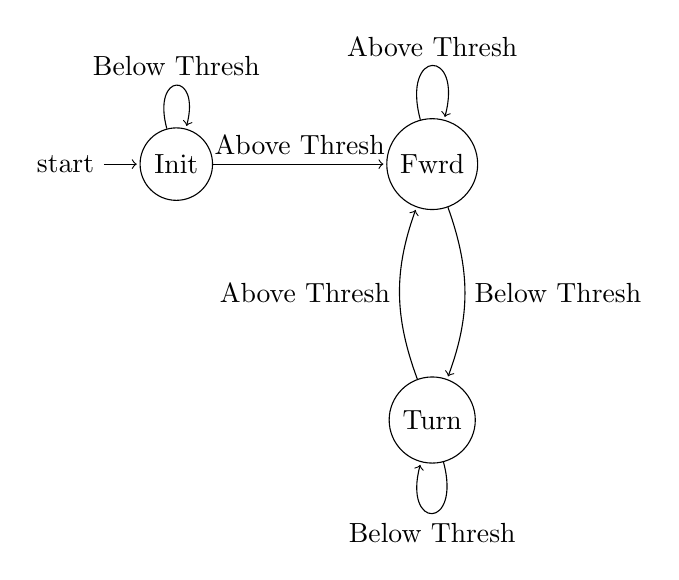
\begin{tikzpicture}[shorten >=1pt,node distance=3.25cm,on grid,auto] 
       \node[state,initial] (Init)   {Init}; 
       \node[state] (Fwrd) [right=of Init] {Fwrd}; 
       \node[state](Turn) [below=of Fwrd] {Turn};
        \path[->] 
        (Init) edge  node {Above Thresh} (Fwrd)
               edge [loop above] node {Below Thresh} ()
        (Fwrd) edge [bend left=20] node  {Below Thresh} (Turn)
               edge [loop above] node {Above Thresh} ()
        (Turn) edge [bend left=20] node {Above Thresh} (Fwrd)
               edge [loop below] node {Below Thresh} ();
    \end{tikzpicture}
    \caption{State Transition Diagram for Racing}
    \label{FSMmain}
\end{figure}

The forward and turn states have a Proportional-Integral-Derivative (PID) controller at their core that controls steering angle; with speed set as a static, open-loop control signal specific to each state. This is described in detail in Section \ref{FSMctrl}.  The purpose of the PID sub-controller is to turn the wheels such that the car remains roughly at the center of the hallway in both the corners and the straight portions of the race course.  In Equation \ref{PIDmainEQ}, the state error of the PID controller is $e(t) = i_{desired} - i_{center}$, with $i_{desired}$ as the position of the target feature (peak) in the scan and $i_{center} = \frac{n}{2}$.  When the desired feature is in the exact center of the scan, the car will be facing that feature.  The position of the peak feature is determined by filtering out the line scan distance readings that fall below the threshold distance.  The average index of the remaining above-threshold readings is the center of the peak feature.  The PID sub-controller attempts to steer towards this.

\begin{equation}
    u(t) = K_P e(t) + K_I \int_{t-T}^{t} e(t) + K_D { d \over dt } e(t) \label{PIDmainEQ}
\end{equation} 

Use of PID control within the FSM controller was found to be vital to successful execution of the racing task.  Making a turn without crashing naturally depends on speed and turning radius, but it also crucially depends on entering the turn at the proper orientation.  At the beginning of PID tuning, we found that there were oscillations in robot trajectory in the straightaways that resulted in the car entering turns pointed either too far into the turn, or to the opposite direction of the turn.  This made turning wildly unpredictable, even for the same tuning parameters of the turn state.  The dynamics of the turn task made it absolutely necessary to dampen oscillations with $K_D$ and to reduce steady-state error with $K_I$.  Typical PID sub-controller outputs are seen in Figure \ref{PIDsuccess}.

\begin{figure}[b]
    \centering
    \includegraphics[width=\columnwidth]{Figures/controlInputs.png}
    \caption{Relative magnitude of the proportional, integral, and derivative control inputs versus time [s] during successful execution of the racing task. Notice the derivative term leads the proportional by approximately 90 degrees, as expected. }
    \label{PIDsuccess}
\end{figure}

\subsection{Drifting}
The choice of drifting or power sliding during the race was a challenging task since sliding the rear wheels perpendicular to their direction of rotation is a highly dynamic maneuver. Small variations in duration of the slide can result in large variations in drift exit trajectory. Due to the highly dynamic and variable nature of power sliding a strategy for achieving adequate tuning was determined and in the end was proven effective. 



First, a manual driving session under radio control was completed. This provided an opportunity to understand the car dynamics and get a feel for the tire friction, vertical center of gravity, side forces during turns at varying speeds, and motor torque capabilities. Second, a heavy focus on tuning the straight away control system to ensure the car entered turns in a repeatable manner with respect to its translation position and heading was completed. This incoming turn repeat-ability provided a critical foundation tuning the actual drift parameters.



Step three was finding the correct time to attempt a power slide. The first attempt at this was based on a distance from the approaching wall, but this quickly was deemed to be a bad indicator of when the actual turn was happening. The final and very effective drift start metric relied on measuring the steering control signal, which would cross a threshold when the car was making a hard right turn and indicate there was sufficient side loading on the tires for a drift to be possible.


Once a start time had been tuned to reliably flag the center of the turn arc where the side loading was highest a "break free" strategy was developed. Initially it wasn't clear whether providing a large negative torque on wheels (hitting the brakes) or a large positive torque (flooring it) would be more effective for breaking the wheels free from the static friction regime. Testing showed that while both approaches were feasible "flooring it" by providing full throttle was more robust to incoming speed variation and also had the nice benefit of keeping the turn velocity high and thus reducing total lap time. 


Consistent drifting around turns with short bursts of full throttle to kick out the rear wheels revealed the need for another control effect; counter steer. In full scale rally car racing drivers will often counter steer, turn the wheel hard in the opposite direction of the turn, to control their yaw rate and prevent over drifting. To achieve consistent drifts a longer slide duration with the addition of counter steer starting after a small delay worked well and ensured the car usually finished turns with a reasonable heading for driving down the next hallway section.

\subsection{Collision Detection and Avoidance}
% - How did we achieve a detection of a collision?
% - What was our strategy for recovering and moving forward
In order to accomplish collision detection and avoidance we implemented a multi-state approach. A collision state was triggered if the robot sensed \textit{k} occluded points out of the \textit{n=100} total points that the robot saw at each time-step. For this system, an occluded point was defined as any point less than \textit{0.5m} away from the robot. The parameter \textit{k} was tuned during testing to only trigger the collision state when a collision had actually happened or was imminent. If the collision state was triggered, the robot would then enter a reverse state in which the robot backs up for a short period to to bring any open space around the obstacle into view of the line scan. After reversing, the robot would then divide its depth scan into two halves (excluding the center portion) and find the side with the highest average depth. It would then lock onto the peak  value of this side as its goal and attempt to navigate to this point as it proceeded forward and around the obstacle. As the robot moves this peak value will obviously change in position with respect to the robot, so the robot would look for this peak value in a window around the index of the scan where it last saw the peak at each time-step, and thus track the furthest depth as it moved forward. Additionally, we added an offset to this furthest point in the direction opposite of the obstacle in order to compensate for the width of the vehicle so that it would not re-collide with the object.

\subsection{Stop Sign Detection}

This challenge was accomplished by developing a custom stop sign detector and implementing it in a ROS nodelet. This nodelet subscribes to the raw RGB color image topic \textit{/camera/color/image\textunderscore{}rect\textunderscore{}raw} published by the custom ROS RealSense node developed for this project. Running in a nodelet allows for zero-copy passing of OpenCV images, speeding the processing on the computationally limited ODROID.

The stop sign detector consists of (1) color thresholding, (2) morphological processing, and (3) blob detection. To visualize the algorithm pipeline, two images are shown for each major process, one with the stop sign on a cluttered desk environment, and one with the stop sign in a straight hallway. The raw RGB imagery are shown in Figures \ref{stopsigndesk}(a) and \ref{stopsignhall}(a).

\begin{figure}[tp]
\begin{center}
\includegraphics[width=.48\textwidth]{Figures/stopsign/stopsign_desk.png}
\caption{Desktop stop sign image as (a) raw RGB, (b) raw HSV, (c) masked by red color thresholding, (d) filled in via closing operation, (e) denoised via erosion operation, and (f) blob detection output from SimpleBlobDetector.}
\label{stopsigndesk}
\end{center}
\end{figure}

\begin{figure}[tp]
\begin{center}
\includegraphics[width=.48\textwidth]{Figures/stopsign/stopsign_hall.png}
\caption{Hallway stop sign image as (a) raw RGB, (b) raw HSV, (c) masked by red color thresholding, (d) filled in via closing operation, (e) denoised via erosion operation, and (f) blob detection output from SimpleBlobDetector.}
\label{stopsignhall}
\end{center}
\end{figure}

Two color masks are used to threshold the image. These masks are in Hue-Saturation-Value (HSV) space rather than Red-Green-Blue (RGB) space. Therefore, the image stream is converted using the \textit{cv::cvtColor} transformation, and the HSV output is represented in RGB space in Figures \ref{stopsigndesk}(b) and \ref{stopsignhall}(b).

\begin{lstlisting}
cvtColor(img_ptr->image, img_hsv, CV_RGB2HSV)
\end{lstlisting}

The two HSV masks are show in Figure \ref{stopsign_color_thresholds}. Since the two HSV thresholds represent the minimum and maximum allowable values, low values of saturation and value were paired with the lowest value of hue. Additionally, red colors reside on both the high end and the low end of the hue spectrum. Therefore, four HSV thresholds must be applied, a minimum and maximum at the low end of the hue spectrum, and a minimum and maximum at the high end of the hue spectrum. 

\begin{lstlisting}
// Masking colors (red orange)
inRange(img_hsv, Scalar(  0, 75, 75), Scalar(  2, 255, 255), mask_red_orange);
// Masking colors (red pink)
inRange(img_hsv, Scalar(178, 75, 75), Scalar(180, 255, 255), mask_red_pink);
// Union two masks to get "red" mask
mask = mask_red_orange | mask_red_pink;
// Apply red mask
bitwise_and(img_hsv, img_hsv, img_hsv_redmasked, mask=mask);
\end{lstlisting}

\begin{figure}[tp]
\begin{center}
\includegraphics[width=.48\textwidth]{Figures/stopsign/stopsign_color_thresholds.png}
\caption{Hue-Saturation-Value thresholds of (left) [2, 75, 75] and (right) [2, 255, 255].}
\label{stopsign_color_thresholds}
\end{center}
\end{figure}

The resulting images from the HSV thresholding are shown in Figures \ref{stopsigndesk}(c) and \ref{stopsignhall}(c).

The threshold operation is not perfect due to sensor noise, glare, and variability in lighting conditions. Therefore, operations must be included to clean up the masked image. This is principally accomplished by morphological processes, specifically a closing operation followed by an opening operation. The closing operation effectively removed holes from the stop sign, since it is a dilation followed by an erosion, as shown in \ref{stopsigndesk} (d) and \ref{stopsignhall} (d). It also increases the blob size of random noise in the image. To eliminate these erroneous blobs, the opening operation erodes and then dilates. Note that the closing operation utilizes a 20 x 20 pixel block while the opening operation only uses a 15 x 15 pixel block. The results of the opening operation are shown in Figure \ref{stopsigndesk}(e) and \ref{stopsignhall}(e).

\begin{lstlisting}
// Define the closing and opening structuring elements
Mat se_closing = getStructuringElement(MORPH_RECT, Size(20, 20));
Mat se_opening = getStructuringElement(MORPH_RECT, Size(15, 15));
// Perform closing then opening
morphologyEx(img_redmasked_binary, mask_close_open, MORPH_CLOSE, se_closing);
morphologyEx(mask_close_open, img_masked_binary_closed_open, MORPH_OPEN, se_opening);
\end{lstlisting}

The results of the morphological processing is a binary image with an octagon-shaped object. Because the color mask and morphological processing yield a clean binary image of the stop sign, a simple blob detector was leveraged. There are several parameters of the \textit{cv::SimpleBlobDetector} class that directly control the accuracy of the stop sign detection. The \textit{filterByCircularity}, \textit{filterByConvexity}, and \textit{filterByArea}  parameters were set to \textit{True}. Since an octagon is similar is shape to a circle, the \textit{minCircularity} was set to 0.75. Additionally, the stop sign is convex, so the \textit{minConvexity} was set to 0.9. Lastly, the \textit{minArea} was set to 1500 pixels, which influences at what distance the stop sign detector is triggered. The output from the blob detector is a circle with the corresponding center and radius of the blob, as shown in Figure \ref{stopsigndesk}(f) and \ref{stopsignhall}(f).

\begin{lstlisting}
// Detect blobs
detector->detect( img_masked_binary_closed_open_inv, keypoints);
// Draw detected blobs as red circles
drawKeypoints( img_blank, keypoints, im_with_keypoints, Scalar(0,0,255), DrawMatchesFlags::DRAW_RICH_KEYPOINTS );
\end{lstlisting}

Once a blob (the stop sign) is detected, the nodelet \textit{std\textunderscore{}msgs::Bool} publisher \textit{stopsign} will change from \textit{False} to \textit{True}. The state machine is always listening to this topic, and will cut throttle immediately for several seconds once the \textit{stopsign} topic is \textit{True}. The \textit{minArea} parameter was tuned such that the car comes to a rolling stop directly at the stop sign.

\section{RESULTS}

\subsection{Timed Trial Runs}
We ran a total of four (4) separate timed trial runs. On the first run we fixed our top speed at \textit{32\%} throttle and the robot succeeded in clocking a time of \textit{17.23s}. This was without any deliberate drifting but seemed to contain some understeer. On the second run we left all parameters the same but on the second turn the understeer was too high and the car chipped the wall. This led to an immediate partial spin of the vehicle but the system was able to recover control and lock back onto the hallway, completing the course in only \textit{19.17s}. On our third run we turned on the drifting mechanism at the second turn but left the top speed at \textit{32\%}. This led to a successful drift at that turn but a slightly longer lap time of \textit{17.66s}, but it also completed our drift challenge requirement for the course. And on our fourth and final run we increased the speed to \textit{34\%} throttle to see if we could improve the total time. This run was very smooth with only slight understeer on the second turn and put in an impressive time of \textit{16.83s} which marked our best time of the day.

\subsection{Stop Sign Detection}
The stop sign detector successfully identified stop signs placed in the path of the robot and triggered the car to autonomously come to a rolling stop. Several tests were carried out, and in all tests, the car successfully came to a rolling stop, paused as if at an intersection, and then continued through the hallway.

\subsection{Collision Detection and Recovery}
This challenge was also passed, but with some difficulty. On our first run, the robot performed well by colliding with the obstacle, reversing, and then following a path safely around the object. However, when we attempted a second trial, the collision with the obstacle was particularly sharp and the RealSense failed which rendered the car blind and so unable to navigate around the object. The first attempt however was enough to pass the challenge requirements.

\section{DISCUSSION}
% Possible discussion topics:
% - The gain tuning tuning process:challenges,  successes, lessons learned, what we would do differently next time
% - Sensing approach: challenges, successes, lessons learned
% - Limitations of our control strategy: works well in the current course, but what would make our control strategy break?

\subsubsection{Control Gain and Parameter Tuning}
One of the most difficult and time consuming processes was tuning our controller gains and algorithm parameters. Each of the control gains and tuning parameters was highly coupled with the speed of the vehicle, which was directly related to the current voltage level of the battery. We were doing open loop control on the forward velocity by setting a reference throttle command. We did not have a method for estimating our vehicle's forward velocity or for measuring the voltage of the battery over time. This made tuning exceptionally challenging as it was hard to get consecutive runs at the same speed. One set of gains would work well for a run or two, and then fail on the next run. For this reason, we wound up tuning four separate sets of control gains for each consecutive run around the course. This worked well for the challenge, but a much better solution would be to estimate the vehicle's forward velocity and do feedback control on the throttle to achieve velocity tracking.

\subsection{Sensors \& Data Processing}
The custom RealSense ROS wrapper proved to be lightweight and reliable. If additional time was allotted for system-level optimization, the car would likely benefit computationally from placing this node in a nodelet and running with a nodelet manager. This would allow for zero-copy passing of the depth image.

\subsubsection{Stop Sign Detection}
While the stop sign detector met the performance criteria well, a few limitations were identified. Firstly, the RealSense D435i camera is configured with auto-exposure, therefore preventing accurate detection during the first five seconds of launching the custom RealSense node. Secondly, glare and poor lighting cause the detector to suffer false negatives. Thirdly, the detector is not foolproof since it does not distinguish the letters \textit{STOP} on the sign. Therefore if the stop sign was blank or said anything else such as \textit{GO}, the detector would suffer a false positive. More generally, red objects that are roughly circular would falsely trigger the detector.

The \textit{minArea} was tuned such that the car would come to a rolling stop by the time it reached the stop sign. Note that this worked for a specific set of parameters including, but not limited to velocity, inertia, and rolling resistance. A more robust method would include active braking, which would stop the car at the stop sign regardless of the system parameters.

Implementing a deep-learning-based object detector such as YOLO was an appealing alternative and the feasibility of such as solution was explored. It was decided that the challenge of installing YOLO and supporting software on the ODROID was not worthwhile. Even if TinyYOLO was successfully running on the ODROID, real-time implementation would have been difficult with the limited computational resources. The filtered blob-detector implementation has the advantage of being computational light in comparison to YOLO, lending itself to real-time operation. If a stronger computational platform was available, YOLO or another deep-learning object detector would likely be the preferred option.

\section{CONCLUSIONS}
Overall, this project can definitely be considered a success. Each challenge was completed successfully. For the stop sign challenge, the robot stopped at the stop sign without incident. Although a few issues were encountered with collision recovery, ultimately tuning of the system provided mostly reliable behavior. Drifting was particularly difficult to tune but also was done with good consistency when it came to validation time. As far as the required time of less than 20 seconds for the course, our system performed admirably. It was very consistent with a best time of \textit{\textasciitilde16.8s}. On one lap it encountered a minor collision with a wall but managed to recover from a slight spin out and still only lost about \textit{2s} off of its time.

Beyond our success on the challenges, our team worked very well together with each member offering a healthy contribution to the overall success of the team. Our meetings were regular and productive with good discussions on options for project direction and techniques to use. In addition to this, much was learned by each member in various areas of robotic design and development. Those of us with little mechanical or electrical experience added to our expertise by being involved in planning and implementing these subsystems. Additionally, those with little experience in ROS or controllers were educated on the practical applications of these techniques via our group discussions and time spent in implementation. In summary, we are fully satisfied with the performance of both our vehicle and our team as a whole.

%%%%%%%%%%%%%%%%%%%%%%%%%%%%%%%%%%%%%%%%%%%%%%%%%%%%%%%%%%%%%%%%%%%%%%%%%%%%%%%%



%%%%%%%%%%%%%%%%%%%%%%%%%%%%%%%%%%%%%%%%%%%%%%%%%%%%%%%%%%%%%%%%%%%%%%%%%%%%%%%%



%%%%%%%%%%%%%%%%%%%%%%%%%%%%%%%%%%%%%%%%%%%%%%%%%%%%%%%%%%%%%%%%%%%%%%%%%%%%%%%%

\section*{APPENDIX}

\subsection{Improving Performance through Deep Learning}
\subsubsection*{Deep Neural Net for State Classification}
One of the initial challenges our team faced was determining how we wanted to handle the turns in the course. Controlling the vehicle around a turn is much different than driving straight down the hallway, and so we decided to handle the control for these two situations independently. In order to update the state machine, different heuristics are applied to the depth line-scan signaling straightaway, pre-turn, and turn states. 

The code and algorithms developed by our team work well at detecting the various states needed to guide the vehicle around a turn. One observation that we made during testing was that the detection of the pre-turn and turn states were dependent on the orientation of the vehicle as it neared a corner. If the vehicle's path was oscillating as it neared a corner, it had the tendency to throw off our corner detector algorithm. As we ramped up the vehicle's speed and added drifting to our control around the corners, it became more and more important to really lock in the exact position in the course that the vehicle should begin executing its turn routine.

We were able to tune our code and algorithms to give us satisfactory performance in the scope of this class. Another route that could be taken is to implement deep learning in an attempt to get more reliable state machine switching. Instead of using the heuristics described above for determining when to switch states, one could apply a deep neural net to the line-scan and use it as a classifier for the vehicle states. As detailed in Section \ref{crtlAppendix}, only portions of the line scan are used to determine the transitioning of the states. The hypothesis presented here is that there is information contained in the line scan that we are discarding which can be used to better differentiate between the different control states. 

\begin{figure}[tp]
\begin{center}
\includegraphics[width=.48\textwidth]{Figures/line_scans.png}
\caption{The plots display examples of line scans taken while traversing the course. The x-axis is the down sampled index of the point in the image space and the y-axis is the distance to the wall. The top two scans are from the vehicle in a straightaway and the bottom two scans are from a turn.}
\label{ls}
\end{center}
\end{figure}

In Figure \ref{ls}, examples of the line scans used for steering control are shown. Each line scan represents the vehicle's distance away from the hallway walls plotted from the left side of the depth image to the right side. The line scans cover about 90 degrees field of view in front of the vehicle and have been down sampled to 100 points. One can see that the scans from different states are significantly different from one another and even have some variance within a state. The goal is to have the neural net learn how to distinguish the vehicle states from the line scan data. Each of the line scan points can be used as an input to a deep neural net. The outputs of the net are the different vehicle states: straight, pre-turn, and turn. The states are mutually exclusive, which makes them conducive to the classification task. Figure \ref{nn} demonstrates the general setup of the proposed neural net.

\begin{figure}[tp]
\begin{center}
\includegraphics[width=.48\textwidth]{Figures/nn.png}
\caption{An example of the general structure for the proposed deep neural net. In our case, the inputs are the points from a line scan, and the outputs are the vehicle states.}
\label{nn}
\end{center}
\end{figure}

The proposed net is composed of one input layer with 100 input nodes, $N$ deep layers, and one output layer with 3 output nodes. When training a similar neural net structure for classifying the MNIST dataset, neural nets with only a single deep layer with the same number of nodes as the input layer were able to achieve 97\% accuracy \cite{aurelion}. For this reason, a reasonable choice for the number of deep layers $N$ is 1-3 layers with 100 nodes each. The more layers that are added will affect the time needed to train the net. Adding more layers also increases the risk of over fitting the data as well. The number of nodes in each deep layer are a hyper-parameter available for tuning, but a reasonable starting point for the deep layers is to have 100 nodes each and be fully connected to the previous layer as seen in Figure \ref{nn}. 

In order to train the network, a significant amount of data would need to be collected over the course of numerous runs around the course. The data that would need to be collected would be the line scans and then a label for each line scan designating which state the vehicle is currently in. We want the vehicle to transition states based on its position in the course, and so one could use a motion capture system to automatically label the line scan dataset (e.g. At +15m in the x direction, the vehicle enters the pre-turn state). In this case, the vehicle could be manually piloted to ensure the vehicle goes through a variety of motions entering the different states to improve the robustness of detection. 


\subsubsection*{Convolutional Neural Net on RGB-D Data for Learning Steering Control}

Another way one could use deep learning to improve vehicle performance would be to try to learn the control signals for the vehicle. Typically, the work flow for control is to sense the environment, use the observations to estimate system states, plan a path forward, and finally generate control commands for executing the trajectory. With advances in deep learning, research groups have been exploring how to compute control signals directly from the sensor observations, effectively streamlining the data flow.

\begin{figure}[h!]
\begin{center}
\includegraphics[width=.45\textwidth]{Figures/conv_net.png}
\caption{This is the convolutional neural net structure employed by Bojarski et al. for their work in end to end learning. }
\label{conv_net}
\end{center}
\end{figure}

The work done by Bojarski et al. in their paper "End to End Learning for Self-Driving Cars", they were able to prove that they could successfully train a convolutional neural network (CNN) on forward facing camera images to learn how to control the steering of the vehicle \cite{bojarski}. Their CNN is composed of 9 layers and they used 72 hours of manual driving data to train the network. The weights for the net were trained by evaluating the mean-square error between the commanded steering angle from the net and the command from the human driver. They concluded that they were able to demonstrate that CNN's are capable of learning the task of road following without any semantic abstraction, lane detection, or path planning. 

Jaritz et al. have expanded on this work in their paper "End-to-End Race Driving with Deep Reinforcement Learning" \cite{jaritz}. They did their work with a rally car simulator and increased the difficulty by including additional control inputs like a hand brake, brake, and throttle. Their deep learning setup differs from Bojarski in that they added a reinforcement learning component by penalizing the car based on its distance away from the center of the course.

Similar to the approach taken by Bojarski, one could use the additional depth information provided by the Realsense RGB-D camera to improve steering control training. Song et al. have begun to explore the realm of applying CNN's to depth images in their paper "Depth CNNs for RGB-D scene recognition: learning from scratch better than transferring from RGB-CNNs"\cite{huang}. The hypothesis here is that depth images provide valuable information in the context of generating steering commands for an autonomous vehicle. It is proposed that CNN structures similar to those used by Bojarski can be applied to depth images. Training takes place by comparing the mean-square error between a manually generated steering command to the steering command generated by the net. 
\begin{figure}[h!]
\begin{center}
\includegraphics[width=.44\textwidth]{Figures/cnn.png}
\caption{Example image taken from Bojarski's paper illustrating how the CNN "sees" a road. The top image is the raw camera image. The bottom left image shows the activation of the first layer of feature maps, while the bottom right shows the activation of the second layer of feature maps.}
\label{cnn}
\end{center}
\end{figure}

\newpage
\subsection{Comparing Two Control Approaches} \label{crtlAppendix}

Over the course of development, two control strategies were explored: PID Feedback Control and finite state machine (FSM).  Both control schemes were successful in navigating the full course without collisions. The differences between the two lie in their performance on the two different types of course section (straights and corners), as well as their speed and ease of implementation. A final useful comparison between the two schemes is the physical difference of the depth camera mounting on the car, Figure 1 shows the camera orientation in both schemes with the right configuration (Figure \ref{fig:single-state}) being PID and the center configuration (Figure \ref{fig:multi-state}) being FSM.

\begin{figure}[h!]
    \centering
    \begin{subfigure}[b]{.45\textwidth}
        \includegraphics[width=\textwidth]{Figures/cam_offset.png}
        \caption{PID Control camera configuration}
        \label{fig:single-state}
    \end{subfigure}
    \begin{subfigure}[b]{.45\textwidth}
        \includegraphics[width=\textwidth]{Figures/cam_centered.png}
        \caption{FSM Control camera configuration}
        \label{fig:multi-state}
    \end{subfigure}
    \caption{Difference in depth camera orientation between the two control schemes}
    \label{fig:camera_config}
\end{figure}

%% ~~~ PID ~~~

\subsubsection{PID Feedback Control}

\begin{figure}[t]
    \centering
    \includegraphics{Figures/emergentTurn.png}
    \caption{A 2D scan of distance readings, angled towards the right, will cause the PID controller to execute a right turn. (Simulated environment, Projected scan points shown in color.)}
    \label{emergentTurn}
\end{figure}

We first attempted Proportional-Integral-Derivative (PID) controller for execution of the entire course.  The camera was mounted horizontally, rotated $-45$\textdegree \ about the vertical (towards the right).  This rotational offset was appropriate because our system is only expected to make right turns.  The control scheme was a single input, single output, feedback controller with the input being a distance metric that was correlated to translation distance from a right side wall.  The controlled parameter is the average of the depth values of the line scan described in Section \ref{lineScan}.  The desired value is some number that conceptually, but not exactly, represents the distance of the car from the right wall of a hallway.  The signal changes proportionally to the distance away from the wall when the vehicle was translated away under a constant heading.   The controller output is a steering angle in $\left[  -\frac{\pi}{4} , +\frac{\pi}{4} \right]$, where values $>0$ point the wheels right.  When the car drifts to the left, the average reading is greater, and the controller steers right to lower this value.  When the car drifts right, the average is lower, and the controller steers left to raise this value.  Car speed was held constant for this scheme by open-loop control of one constant duty cycle of the drive motor.

Given the above,  we assume that if the controller isn't too aggressive then the control output will remain small, the heading changes will remain small, and the controller should stay reasonably stable. The control equation for the steering angle is below:  

\begin{equation}
    u(t) = K_P e(t) + K_I \int_{t-T}^{t} e(t) + K_D { d \over dt } e(t)
\end{equation} \label{PIDeq}

The integral of error is calculated using the rectangular approximation from a specified past horizon until the present time-step.  The derivative of error is calculated as an average slope between a specified time horizon in the past and the present time-step. 

The PID controller has a surprising emergent behavior in that it causes the car to correctly make right turns without any modification whatsoever. No special cases or context-dependent gains are required.  As the car approaches a corner, the left-most samples of the scan begin to fall onto the left wall around the corner, and thus have much higher distance readings than those striking the nearest walls.  (Figure \ref{emergentTurn})   This raises the average value of the line scan.  In response, the controller outputs an increasingly right turn, as though the right wall were rapidly drifting away.  The result is that the car makes the right turn.  As soon as the turn is completed the line scan samples from the right wall of the new straightaway, now much closer, and the controller corrects trajectory to forward driving.  It is possible to choose a proportional gain $K_P$ that is aggressive enough to correctly make right turns of the course, but not aggressive enough to erroneously steer the car into the entry recesses of the various labs.  In fact, the integral and derivative controller terms were not necessary at slow speeds, and the course can be completed on proportional control alone in under a minute.

The strongest benefit of this approach was its simplicity and speed of implementation and tuning. With a single set of gains a controller was found that could be handle both turns and straightaways. The largest negative was that by following the right side wall the input signal was disturbed by the doorways and alcoves on the right.  These perturbations limited the feasible top speed for the PID scheme and motivated the investigation of the FSM scheme.  Also, the left walls of straightaways and the oncoming walls of corners are relevant to effective turning and drifting at high speed.  (See Section \ref{FSMctrl})  These features are not adequately handled by the PID controller.

%% ~~~ FSM ~~~

% - What a priori knowledge did we use to our advantage?
% - What parts of the course added difficulty and why? (e.g. corners, alcoves, the workspace area by the stairs, etc)
% - Decision to go with a state machine for handling the course and reasons why (relate back to different sections of the course having unique control objectives)
% - Address the straightaway state, the pre-turn state, the turn state, and finally the transition back to the straightaway state

\subsubsection{Finite State Machine} \label{FSMctrl}

\tikzset{
    ->,
    >=latex,
}

\begin{figure}[t]
    \centering
    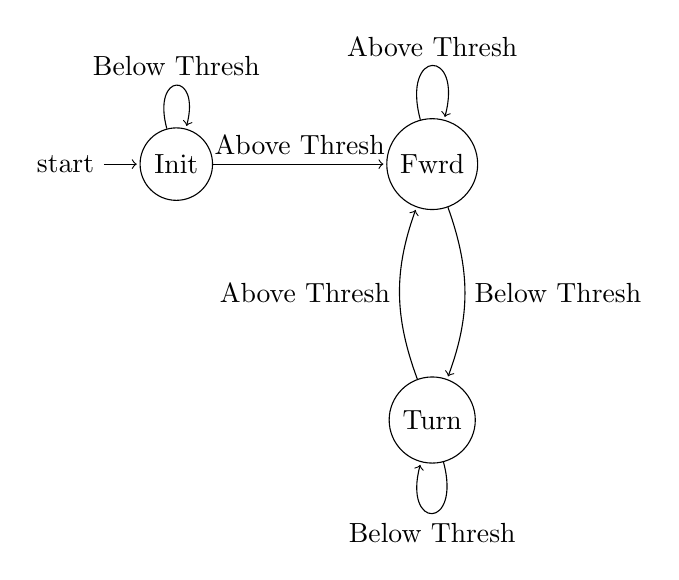
\begin{tikzpicture}[shorten >=1pt,node distance=3.25cm,on grid,auto] 
       \node[state,initial] (Init)   {Init}; 
       \node[state] (Fwrd) [right=of Init] {Fwrd}; 
       \node[state](Turn) [below=of Fwrd] {Turn};
        \path[->] 
        (Init) edge  node {Above Thresh} (Fwrd)
               edge [loop above] node {Below Thresh} ()
        (Fwrd) edge [bend left=20] node  {Below Thresh} (Turn)
               edge [loop above] node {Above Thresh} ()
        (Turn) edge [bend left=20] node {Above Thresh} (Fwrd)
               edge [loop below] node {Below Thresh} ();
    \end{tikzpicture}
    \caption{State Transition Diagram for Racing}
    \label{FSMrace}
\end{figure}

The finite state machine was the most successful and flexible of the two controllers implemented.

Each state represents an operating mode in which an appropriate controller is active.  Transitions represent conditions that trigger a switch to a different operating mode.  The FSM is implemented as its own ROS Python node. An overview of the FSM controller for the racing task can be seen in Figure \ref{FSMrace}.  Every time-step, the current state controller takes the following steps:

\begin{enumerate}
    \item Evaluate sensor data and make appropriate calculations
    \item Apply control effort
    \item Evaluate transition conditions 
    \item Set next state
\end{enumerate}

The primary criterion for state transitions is a threshold on the number of distance readings of the line scan above a specified value.  In a line scan of $n$ readings, if $m$ or more readings are greater than distance $d$, then the ``Above Thresh'' condition is met (Figure \ref{FSMrace}), otherwise the condition is considered ``Below Thresh''.  The threshold distance $d$ is different for each turn of the course, because the radii of the turns are different.

In the initial state, speed and steering angle outputs are set to zero.  In this state the system is waiting for an unobstructed straight hallway to begin driving.  If this condition is not met, the car continues to idle.  If it is met, then control transitions to the forward state.

Both the forward and turning states use a PID sub-controller to calculate steering commands to try to center the peak of distances from the depth line scan within its view.  In the FSM scheme, the state error of the PID controller is $e(t) = i_{desired} - i_{center}$, with $i_{desired}$ as the position of the target feature (peak) in the scan and $i_{center} = \frac{n}{2}$.  When the desired feature is in the exact center of the scan, the car will be facing that feature.  When the car is within $\pm$ 30 degrees of a parallel to the hallway heading the line scan provides a natural peak of distances correlating to the center of the hallway ahead. This ``center peak'' provides an easy target for a control signal and can be shown in blue and red in Figure \ref{redPoints}. The red points indicate the distance value was greater than a target threshold and its position is used in the average that the controller will try to center in its view.  Note that the camera is mounted facing directly forward for the the FSM control scheme, and there is no angular offset as was used for the PID control method.

\begin{figure}[h]
    \centering
    \includegraphics[width=\columnwidth]{Figures/redPeak.png}
    \caption{Binned line scan distances [m] versus index, with above-threshold values highlighted in red.}
    \label{redPoints}
\end{figure}

The purpose of the forward state is straight driving at high speed, keeping the car centered in the hallway using the scan peak-seeking control behavior described above.  The forward state monitors the oncoming flat wall which triggers a transition to the turn state when the \textit{Above Thresh} condition is no longer met.

Control within the turn state is similar to the forward state, but with a small change that produces a turning behavior.  Straight-line driving continues at the beginning of the turn state, but with a corner detection filter enabled.  When the filter detects a corner the vehicle begins a right turn, which continues until the distance peak of an open hallway ahead appears in view.  When this happens, a transition to the forward state is triggered by the \textit{Above Thresh} condition.  Drifting (power-sliding) is also handled by the turn state, as described above in the main report.

The forward and turn states handle all controls for the racing task.  The PID sub-controllers within each state provide a steering signal only.  The speed is statically set at each state as a faction of 100\% duty cycle of the drive motor.  Speed control is open loop, and the actual speed depends heavily upon battery voltage.  Collision avoidance and vision are described above in the main report.

There are several advantages to the FSM control scheme.  The first is encapsulation.  Each state controller may be written independently with only one control scheme per state.  Transitions are deterministic given specific sensor readings, and are explicitly defined.  Another benefit is that the forward camera mounting yields an input signal that is clean and largely unaffected by things like doorways on the side of the hallway.  These troublesome features appear in the periphery of the horizontal FOV, and do not obscure the central peak of the line scan that is critical for control. 

However, the finite state machine is not without disadvantages.  The first is that assumptions about state transitions are built into the system.  That is, if the controller for the current state is no longer appropriate for real-world conditions, and there are no conditions to match this change, then the system will continue to apply inappropriate control without hope of recovery.  There is no learned or adaptive re-routing of state transitions implemented.  This burdens the system designer with the responsibility of carefully tuning transition conditions that handle noisy data and a distribution of car orientations.  Another downside is the need for multiple discrete states, since the forward driving scheme alone does not properly handle the opening of a right-corner and steer towards it.  An important assumption of the FSM scheme is that the trajectory leading into the right turn is stable and has only small disturbances.  This was only true after laborious tuning of the forward controller parameters.

\subsubsection*{Overall Performance Comparison}
While the PID control scheme had the benefit of rapid implementation and minimal tuning, the FSM control scheme allowed for a \textit{much} higher course speed due to the better control signal dynamics on the long straight sections.  The FSM control scheme required much more tuning and implementation time.  We were able to save some time by using a simulator, and by systematically and effectively breaking testing into discrete test.

%\begin{figure}[h]
 %   \centering
 %   \begin{subfigure}[b]{.45\textwidth}
 %       \includegraphics[width=\textwidth]{Figures/cam_offset.png}
 %       \caption{Course and camera rays from simulator}
 %       \label{fig:rays}
 %   \end{subfigure}
 %   \begin{subfigure}[b]{.45\textwidth}
 %       \includegraphics[width=\textwidth]{Figures/cam_centered.png}
 %       \caption{Depth line-scan showing distance peak}
 %       \label{fig:depthscan}
 %   \end{subfigure}
%    \caption{MSC input signal visualizations}
%    \label{fig:msc_signals}
%\end{figure}

\addtolength{\textheight}{-12cm}   % This command serves to balance the column lengths
                                  % on the last page of the document manually. It shortens
                                  % the textheight of the last page by a suitable amount.
                                  % This command does not take effect until the next page
                                  % so it should come on the page before the last. Make
                                  % sure that you do not shorten the textheight too much.

\begin{thebibliography}{99}
\bibitem{HAREproject} https://github.com/erush91/HARE.git

\bibitem{aurelion} Geron, Aurelien. "Chapter 10: Introduction to Artificial Neural Networks." Hands-On Machine Learning with Scikit-Learn ; TensorFlow, O'Reilly Media, Inc., 2017, pp. 255-276.

\bibitem{jaritz} M. Jaritz, R. de Charette, M. Toromanoff, E. Perot, and F. Nashashibi.  End-to-End Race Driving with Deep Reinforcement Learning

\bibitem{bojarski} M. Bojarski, D. Del Testa, D. Dworakowski, B. Firner, B. Flepp, P. Goyal, L. D. Jackel, M. Monfort, U. Muller, J. Zhang, et al. End to end learning for self-driving cars. arXiv preprint arXiv:1604.07316, 2016.

\bibitem{huang} J. Huang and D Altamar. Pose Estimation on Depth Images with Convolutional Neural Network

\bibitem{AutoRally} https://autorally.github.io/

\bibitem{BARC} http://www.barc-project.com/

\bibitem{RACECAR} https://mit-racecar.github.io/





\end{thebibliography}




\end{document}

